\chapter{CHIẾN LƯỢC VÀ BACKTEST}
\section{Thiết kế chiến lược}
P3 chuyển xác suất chữ số thành các pool năm vị trí, rồi sinh vé bằng tích Descartes. Ba cấu hình được kiểm thử là $2\times2\times2\times2\times2=32$ vé, $3\times2\times2\times2\times1=24$ vé và $3\times3\times2\times1\times1=18$ vé mỗi ngày. Một nhánh riêng tập trung vào giải Bảy: chọn các tiền tố đứng đầu ở ba vị trí đầu và thử $m=1,\ldots,10$ đuôi số đứng đầu ở hai vị trí cuối.

Mỗi vé có giá 10.000 VND. Kết quả được đối sánh với toàn bộ 27 giải năm chữ số trong ngày; một vé có thể nhận nhiều giải hợp lệ. Mức trả trong code backtest là: Phụ Đặc biệt 25.000.000; Khuyến khích Đặc biệt 40.000; giải Nhất 10.000.000; Nhì 5.000.000; Ba 1.000.000; Tư 400.000; Năm 200.000; Sáu 100.000; Bảy 40.000 VND.

\section{Chia tập và chỉ số}
Validation 2023--2024 dùng để so sánh ứng viên; final test 2025--2026 chỉ được mở một lần cho đánh giá cuối. Lợi nhuận ngày là
\[
\Pi_t=\sum_{g\in G_t}R_g-10\,000 n_t,
\]
trong đó $G_t$ là tập giải vé nhận được, $R_g$ là tiền trả của giải và $n_t$ là số vé. ROI bằng tổng lợi nhuận chia tổng chi phí. Cách tính này tránh áp dụng một công thức hòa vốn duy nhất cho các chiến lược có cơ cấu giải khác nhau.

\section{Kết quả P3}
\begin{table}[H]\centering\small
\caption{Backtest các cấu hình pool năm chữ số}\label{tab:p3-summary}
\begin{tabular}{llrrrr}\toprule
Fold & Cấu hình & Số ngày & Số vé & Lợi nhuận (VND) & ROI\\\midrule
Validation & 32 vé & 723 & 23136 & -143.600.000 & -62,07\%\\
Validation & 24 vé & 723 & 17352 & -134.120.000 & -77,29\%\\
Validation & 18 vé & 723 & 13014 & -104.580.000 & -80,36\%\\
Final test & 32 vé & 606 & 19392 & -147.120.000 & -75,87\%\\
Final test & 24 vé & 606 & 14544 & -110.000.000 & -75,63\%\\
Final test & 18 vé & 606 & 10908 & -86.940.000 & -79,70\%\\\bottomrule
\end{tabular}\end{table}

\begin{figure}[H]\centering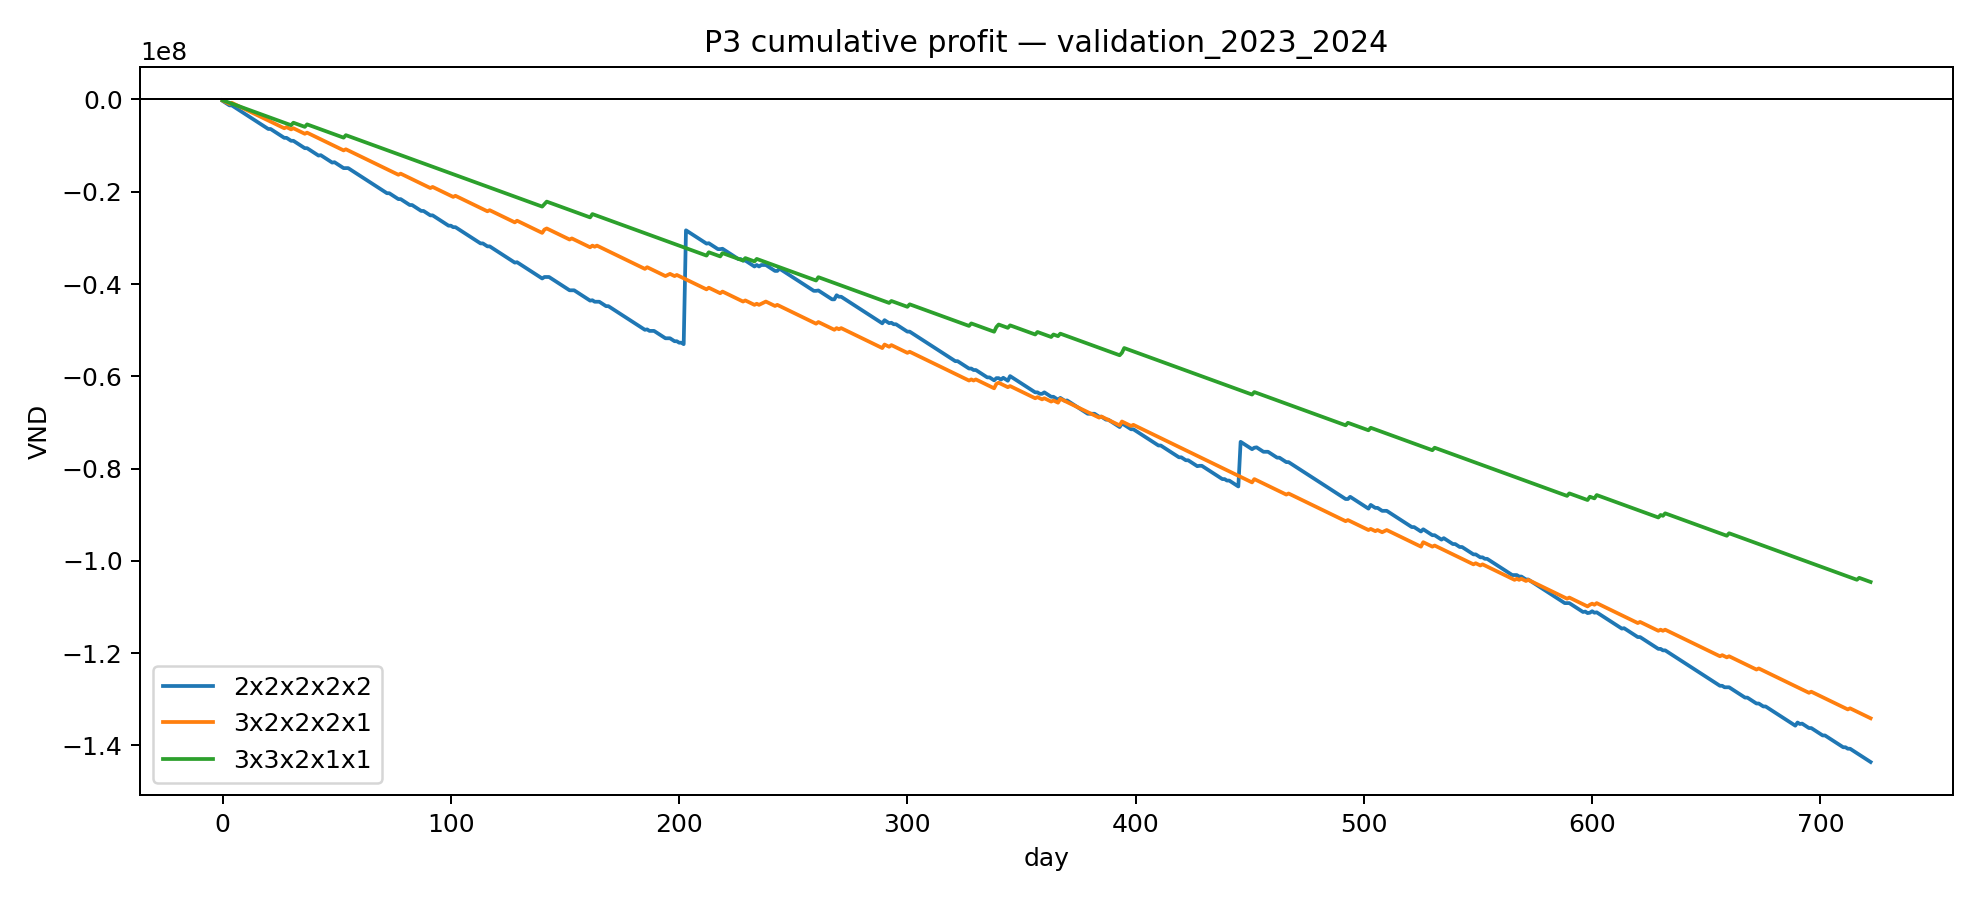
\includegraphics[width=0.92\linewidth]{../artifacts/p3_strategies/cumulative_profit_validation_2023_2024.png}\caption{Lợi nhuận tích lũy của các pool trên validation.}\end{figure}
\begin{figure}[H]\centering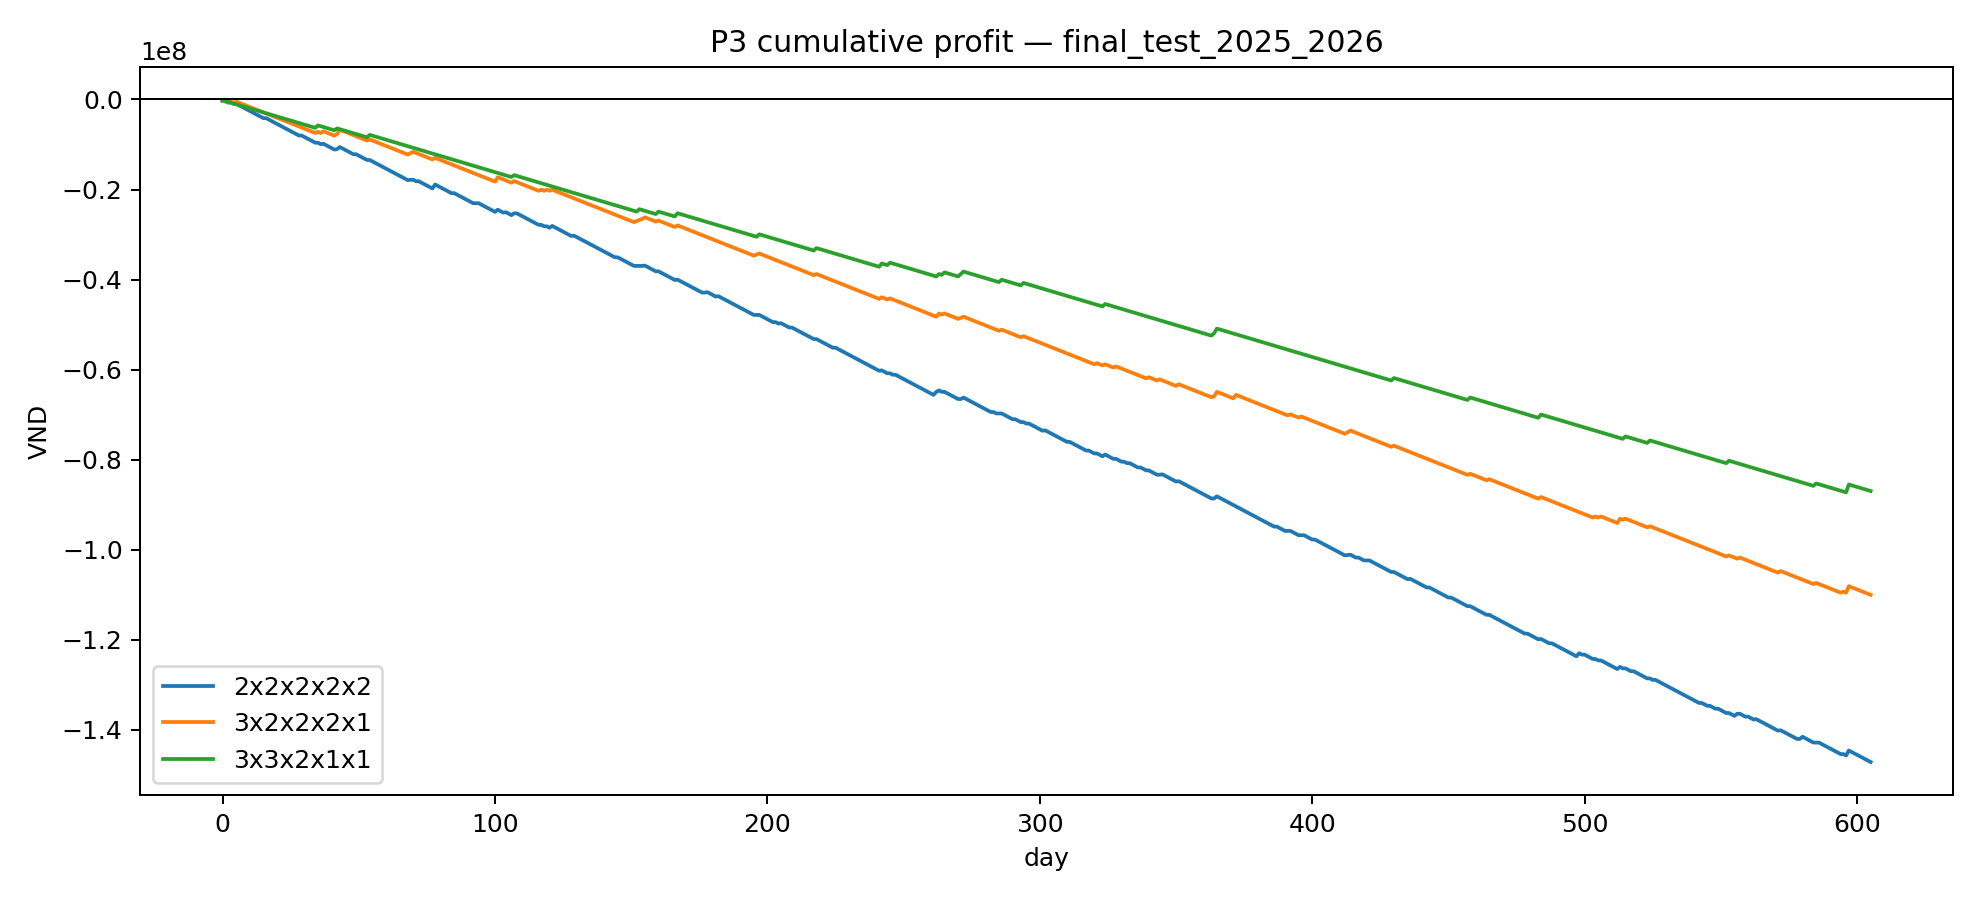
\includegraphics[width=0.92\linewidth]{../artifacts/p3_strategies/cumulative_profit_final_test_2025_2026.png}\caption{Lợi nhuận tích lũy của các pool trên final test.}\end{figure}

\section{Chiến lược giải Bảy theo $m$}
Kết quả theo $m$ được giữ lại như một thí nghiệm độ nhạy. Việc tăng $m$ làm tăng số lựa chọn và chi phí, nhưng không bảo đảm tăng lợi nhuận; do đó, cấu hình tốt nhất phải được khóa từ validation trước khi xem final test.
\begin{figure}[H]\centering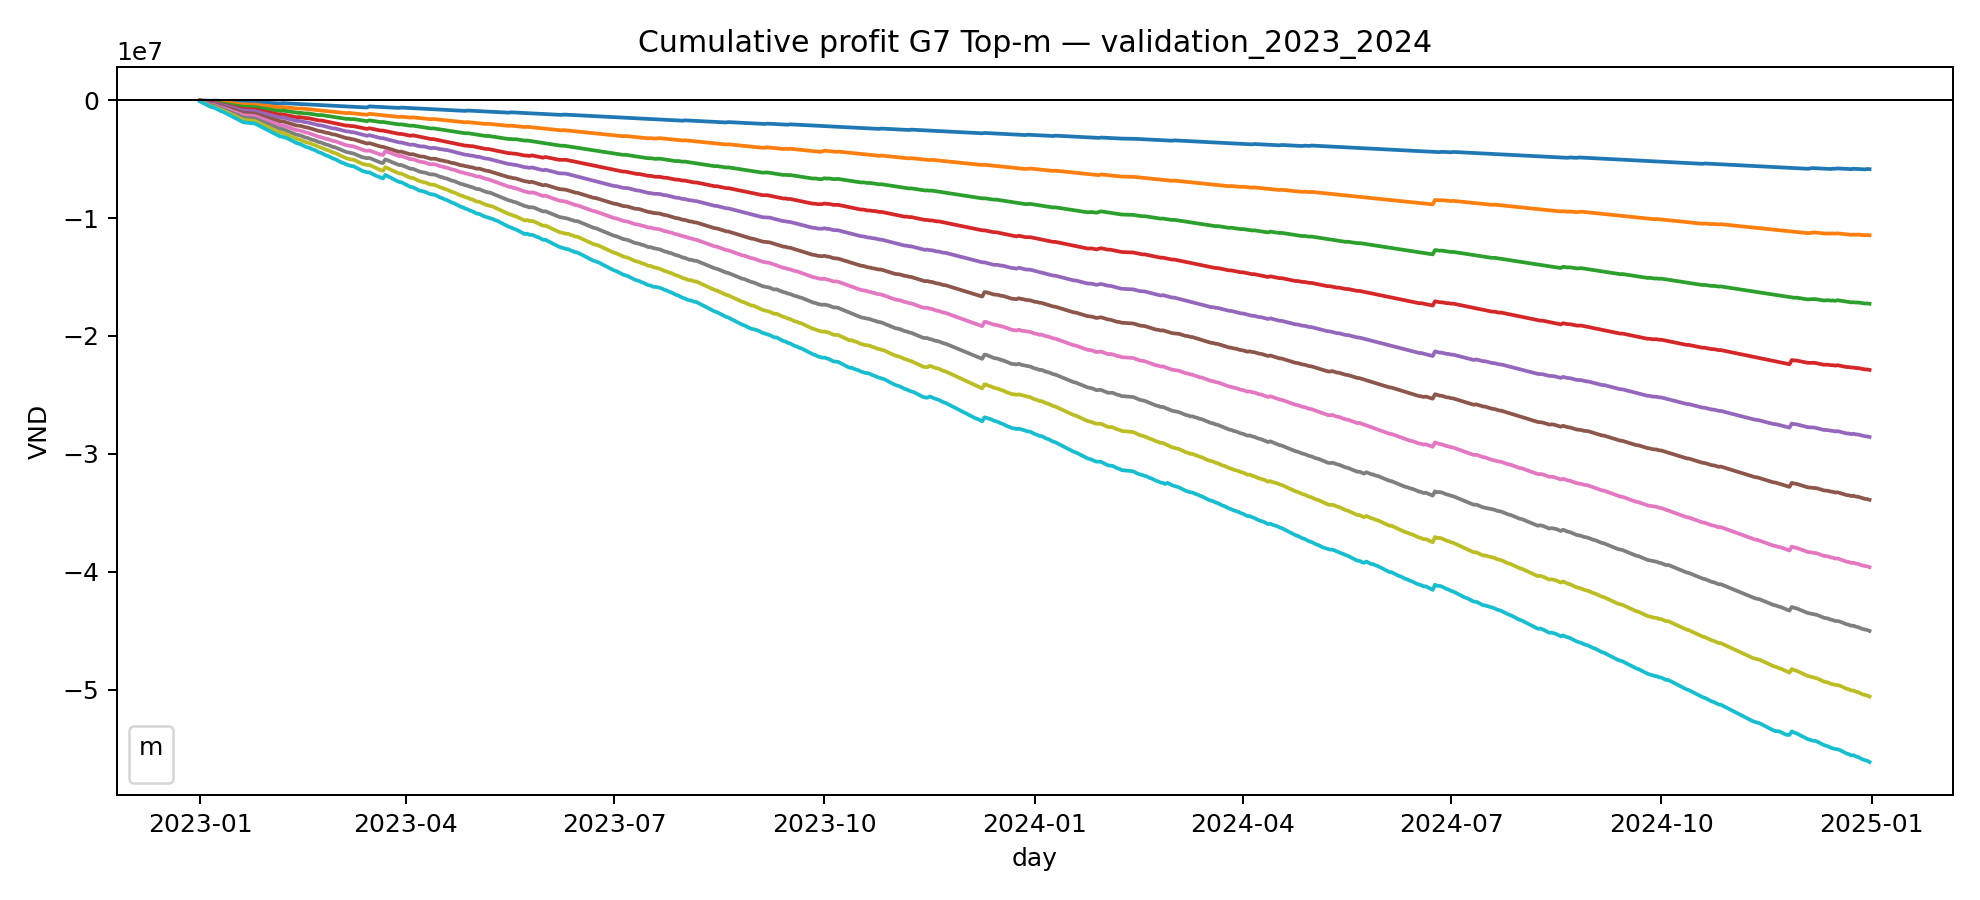
\includegraphics[width=0.92\linewidth]{../artifacts/p3_strategies/g7_topm_prefix/cumulative_profit_validation_2023_2024.png}\caption{Lợi nhuận tích lũy của chiến lược tập trung giải Bảy trên validation.}\end{figure}
\begin{figure}[H]\centering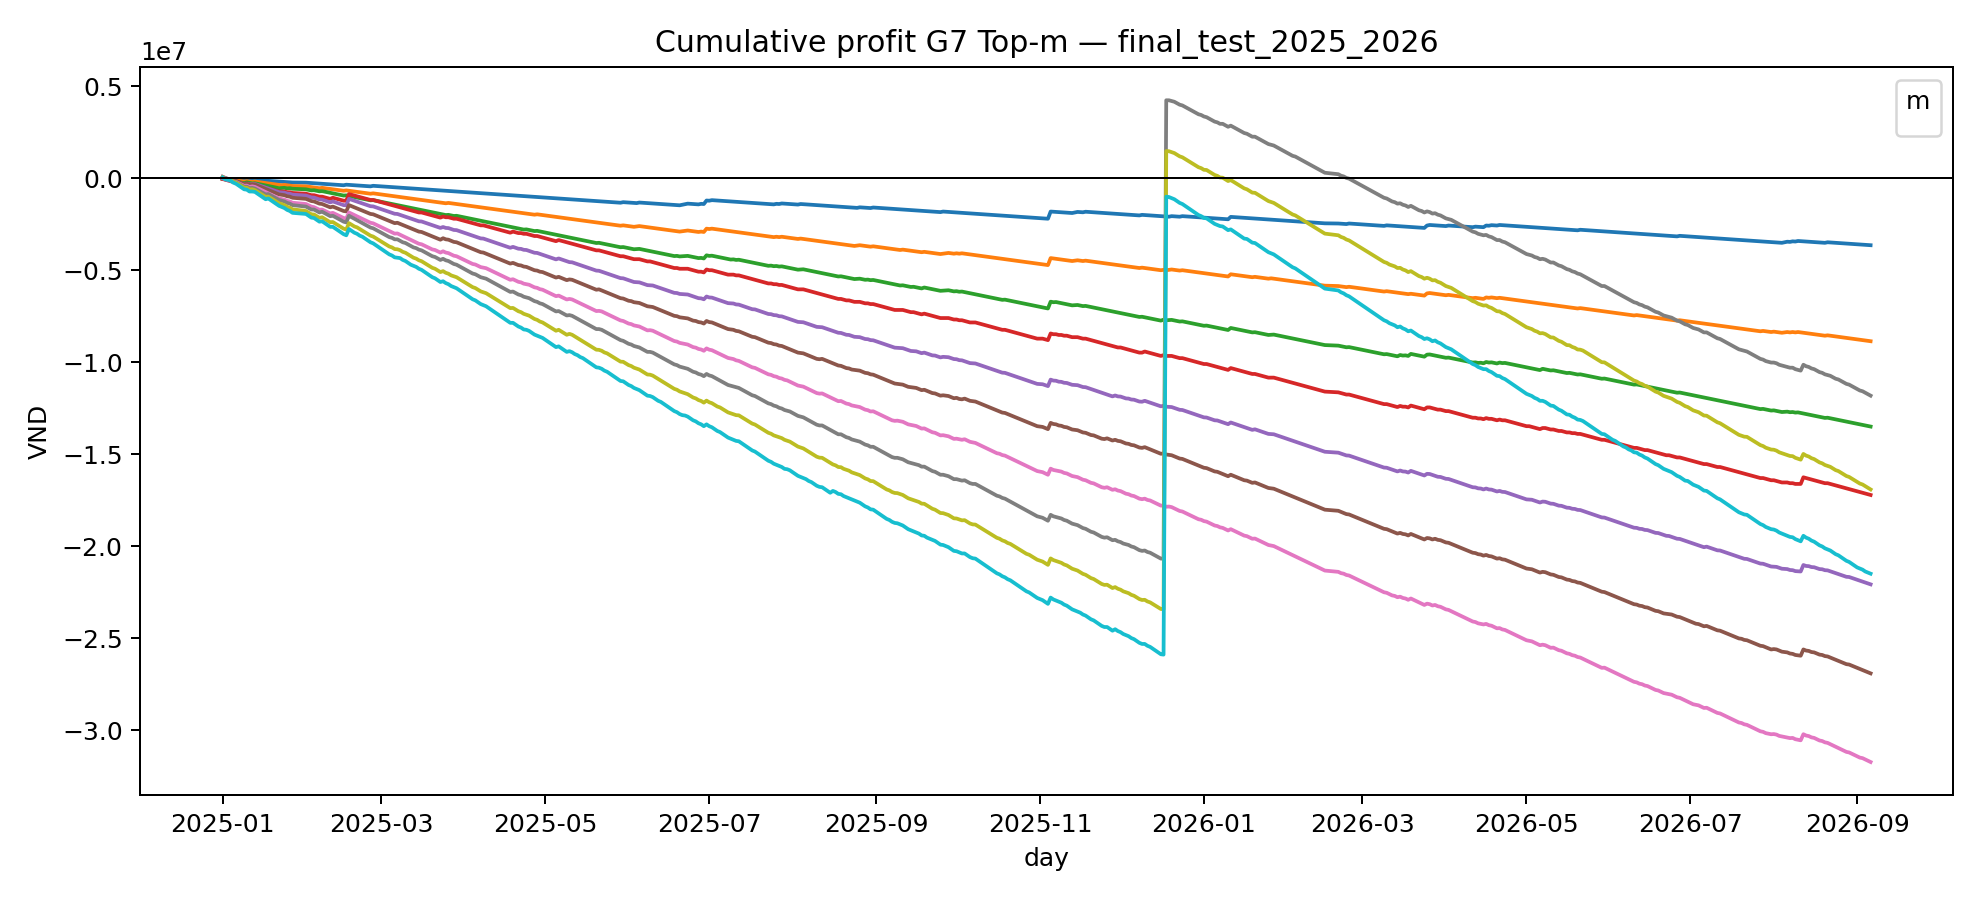
\includegraphics[width=0.92\linewidth]{../artifacts/p3_strategies/g7_topm_prefix/cumulative_profit_final_test_2025_2026.png}\caption{Lợi nhuận tích lũy của chiến lược tập trung giải Bảy trên final test.}\end{figure}
\begin{figure}[H]\centering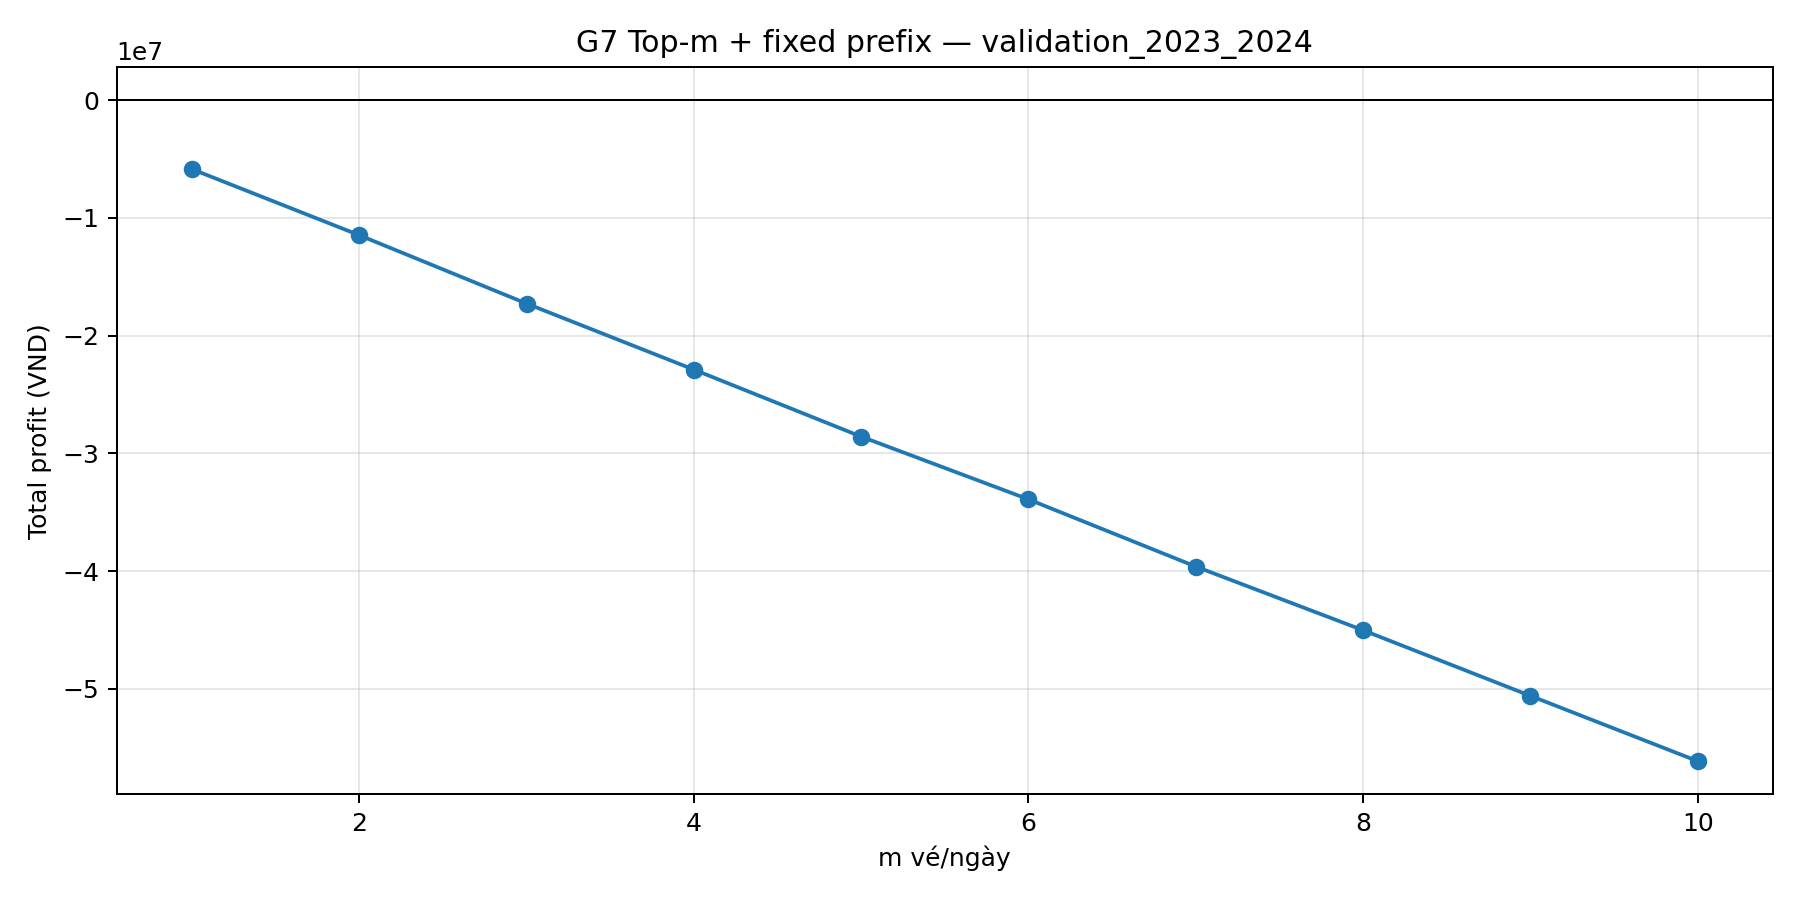
\includegraphics[width=0.92\linewidth]{../artifacts/p3_strategies/g7_topm_prefix/profit_by_m_validation_2023_2024.png}\caption{Độ nhạy lợi nhuận theo số đuôi $m$ trên validation.}\end{figure}
\begin{figure}[H]\centering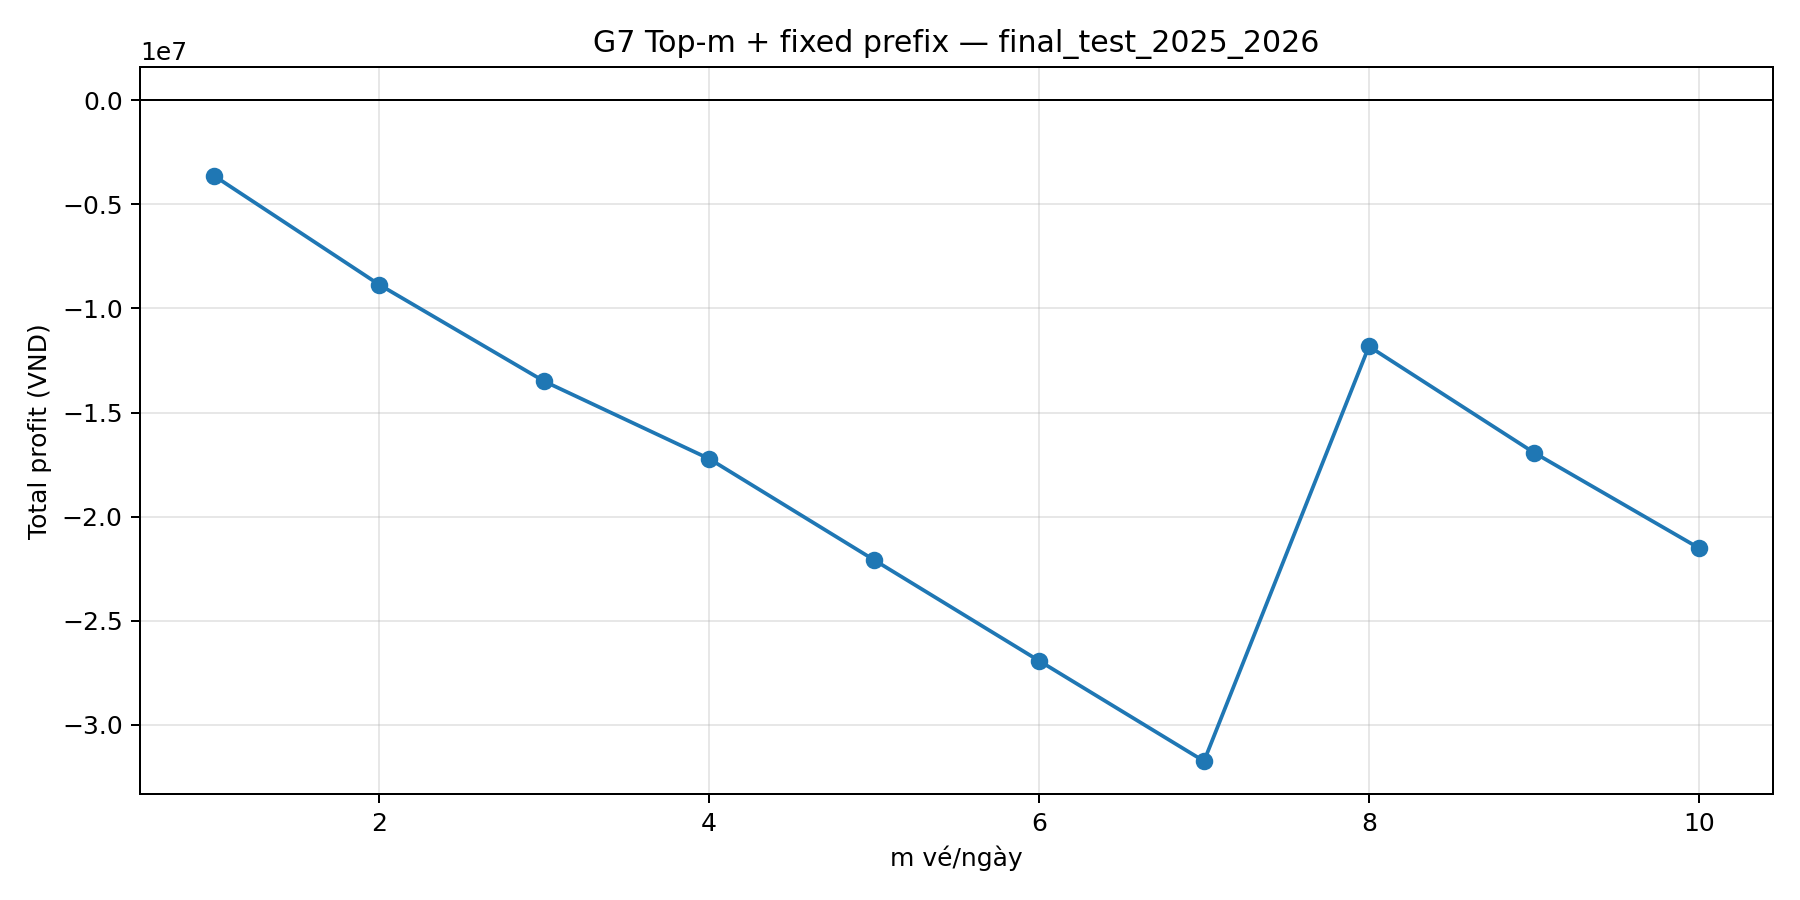
\includegraphics[width=0.92\linewidth]{../artifacts/p3_strategies/g7_topm_prefix/profit_by_m_final_test_2025_2026.png}\caption{Độ nhạy lợi nhuận theo số đuôi $m$ trên final test.}\end{figure}

\section{Diễn giải}
Tất cả cấu hình đều có ROI âm trên cả hai giai đoạn. Cấu hình 32 vé có tỷ lệ ngày có ít nhất một lần trúng cao hơn, nhưng chi phí cũng lớn hơn và tổng lợi nhuận vẫn âm. Đây là bằng chứng trực tiếp rằng một cải thiện nhỏ về thứ hạng chữ số trong P2 không chuyển thành lợi thế kinh tế trong cơ chế trả thưởng được mô phỏng.
